\chapter{Binarizzazione di immagini}
\label{chap:image-binarization}


\section{Introduzione}
Nel campo dell'\textit{image processing} ricopre un ruolo fondamentale la possibilit\`a di distinguere diversi oggetti, forme e contorni presenti nell'immagine in analisi. Per far ci\`o \`e possibile ricorrere a svariate metodologie, che sono strettamente dipendenti dal contesto in cui si intende operare. Per esempio, nel caso del \textit{riconoscimento ottico dei caratteri} (OCR), le operazioni che andranno descritte assumono importanza assoluta, dato che questo tipo di applicazione, per operare al meglio, ha spesso bisogno di ricevere in input un'immagine in bianco e nero, in cui lo sfondo \`e di colore bianco e il testo \`e di colore nero. Gli argomenti affrontati, nel caso di un'applicazione OCR, saranno soprattutto utili nel caso in cui il motore utilizzato sia \textit{open-source} (vedi \textit{Tesseract}), ovvero nel caso in cui un buon \textit{pre-processing} dell'immagine possa fare la differenza. In questo articolo andremo quindi ad analizzare gli \textit{algoritmi} pi\`u ricorrenti nell'ambito del \textit{thresholding} di immagini e nella sezione \ref{sec:image-bin-proposed-approach} affronteremo un approccio specificamente studiato per i casi d'uso della libreria QI-OCR.

Da qui in avanti ipotizzeremo di lavorare con immagini originali in \textit{scala di grigi} con profondit\`a 8 bit, anche se i metodi descritti possono facilmente essere generalizzati per immagini con pi\`u di un canale colore.


\section{Sogliatura globale}
\`E il pi\`u semplice metodo di \textit{thresholding}, che prevede la scelta di un determinato valore di soglia, compreso tra 0 e 255. L'algoritmo di sogliatura prevede quindi la scansione, pixel per pixel, dell'immagine e, nel caso in cui il valore del pixel esaminato sia minore del valore di soglia, tale pixel assumer\`a valore zero, che corrisponde al colore nero. Altrimenti, nel caso in cui il valore del pixel esaminato sia maggiore o uguale del valore di soglia, tale pixel assumer\`a valore 255, che corrisponde al colore bianco. Risulta facile intuire quale possa essere il problema principale di questo tipo di algoritmo di sogliatura, ovvero la scelta del valore di soglia.
Nel caso in cui il contesto in cui si opera sia relativamente statico, la \textit{sogliatura globale} risulta comunque l'opzione pi\`u consigliata, per la sua facilit\`a di implementazione. In particolare, il metodo descritto risulta adatto se le immagini in analisi presentano all'incirca caratteristiche uniformi in termini di illuminazione e contrasto. Se cos\`i non fosse, sarebbe necessario valutare l'implementazione di algoritmi leggermente pi\`u complessi.
\begin{algorithm}
	\caption{Sogliatura globale}
	\label{alg:thresh-global}
	\begin{algorithmic}[1]
		\Function{global-thresholding}{}
			\State $\vars{image} \gets \text{input image}$
			\State $\vars{thresh} \gets \text{threshold value}$
			
			\For {$\vars{i} \text{ in \textproc{rows}(\vars{image})}$}
				\For {$\vars{j} \text{ in \textproc{columns}(\vars{image})}$}
					\If {$\vars{image[i][j]} \geq \vars{thresh}$}
						\State $\vars{image[i][j]} \gets 255$
					\Else
						\State $\vars{image[i][j]} \gets 0$
					\EndIf
				\EndFor
			\EndFor

			\Return $\vars{image}$
		\EndFunction
	\end{algorithmic}
\end{algorithm}


\section{Sogliatura adattativa (o locale)}
Questo metodo di \textit{thresholding} consente di sopperire alle mancanze della sogliatura globale, nel caso in cui le immagini in analisi presentino illuminazione e/o contrasto non uniforme. In particolare, questa tecnica dinamica computa automaticamente differenti valori di soglia per diverse aree dell'immagine. Dunque, l'immagine viene suddivisa in tante \textit{sotto-immagini}, abbastanza piccole da poter ipotizzare che in ciascuna illuminazione e contrasto siano sufficientemente uniformi. Una volta partizionata l'immagine, un valore di soglia viene calcolato per ciascuna \textit{finestra}. Il calcolo di ogni valore di soglia dipende dall'implementazione specifica dell'algoritmo, ma genericamente si ricorre all'utilizzo, per ogni sotto-immagine, di semplici operatori statistici, come la media, la mediana o la media fra massimo e minimo.\par
Alcune tecniche di sogliatura locale efficaci sono implementate da algoritmi quali quello di \textit{Niblack}\cite{bib:niblack} e \textit{Sauvola}\cite{bib:sauvola}. In particolare, l'algoritmo di \textit{Niblack} prevede l'utilizzo delle metriche di media e deviazione standard, per una specifica finestra centrata su ciascun pixel dell'immagine. La formula utilizzata per calcolare un generico valore di soglia \`e data da:
\begin{equation}
	\label{eq:niblack}
	T(x, y) = m(x, y) + k \cdot s(x, y),
\end{equation}
dove $T(x, y)$ indica il valore di soglia per il pixel in posizione $(x, y)$, $m(x, y)$ ($s(x, y)$) indica la media (deviazione standard) dei valori dei pixel vicini a quello centrato sulla finestra corrente e $k$ \`e un coefficiente, che pu\`o essere determinato empiricamente\footnote{\textit{Niblack} consiglia l'impostazione del parametro $k$ al valore $-0.2$.}.\par
L'utilizzo di parametri configurabili \`e molto comune per algoritmi di questo tipo, in quanto questi risultano essere fortemente dipendenti dal contesto di utilizzo. Un esempio pratico riguarda la libreria \textit{OpenCV}, che nella funzione $\textproc{adaptiveThreshold}$ consente di selezionare un valore $c$, che viene sottratto da ciascun valore di soglia di ogni sotto-immagine. Per esempio, nel caso in cui il valore di soglia venga calcolato utilizzando la media $mean$, il limite scelto non sar\`a esattamente $mean$, ma $mean - c$.

\par
Purtroppo, il problema principale della sogliatura adattativa \`e che tende a valorizzare tutti gli elementi presenti nell'immagine, non consentendo di differenziare al meglio le componenti d'interesse da quelle che invece si vorrebbero scartare.
\begin{algorithm}
	\caption{Sogliatura adattativa}
	\label{alg:thresh-local}
	\begin{algorithmic}[1]
		\Function{local-thresholding}{}
			\State $\vars{image} \gets \text{input image}$
			
			\For {$\vars{pixel} \text{ in \vars{image}}$}
				\State $\vars{thresh} \gets \textproc{statistical-operator(\textproc{neighbors(pixel)})}$
				\If {$\vars{pixel} \geq \vars{thresh}$}
					\State $\vars{pixel} \gets 255$
				\Else
					\State $\vars{pixel} \gets 0$
				\EndIf
			\EndFor

			\Return $\vars{image}$
		\EndFunction
	\end{algorithmic}
\end{algorithm}

\section{Sogliatura di Otsu}
Questo tipo di sogliatura utilizza tecniche di analisi dell'\textit{istogramma}\footnote{L'\textit{istogramma} $h$ di un'immagine $I$ in scala di grigi, con valori d'intensit\`a $\in [0, K - 1]$ e definiti nell'immagine della funzione $I$,  \`e una funzione tale che $h(i)$ \`e uguale al numero di pixel di $I$ con valore di intensit\`a $i$, per $0 \leq i < K$. Pi\`u formalmente $h(i)=|{(u, v)\colon I(u, v)=i}|$.} dell'immagine ed \`e particolarmente adatto per immagini \textit{bimodali} (vedi figura \ref{fig:bimodal-hist}), ovvero per immagini che presentano istogrammi con una netta separazione tra due picchi principali. La binarizzazione di \textit{Otsu} si occupa proprio di trovare la "valle" di scissione fra tali picchi, che risulta essere proprio il valore di soglia ottimale per l'applicazione di un'operazione di sogliatura globale.\par
\pgfplotsset{compat=1.16,width=13cm,height=7cm}
\begin{figure}[t]
	\centering
	\resizebox{13cm}{7cm}{%
		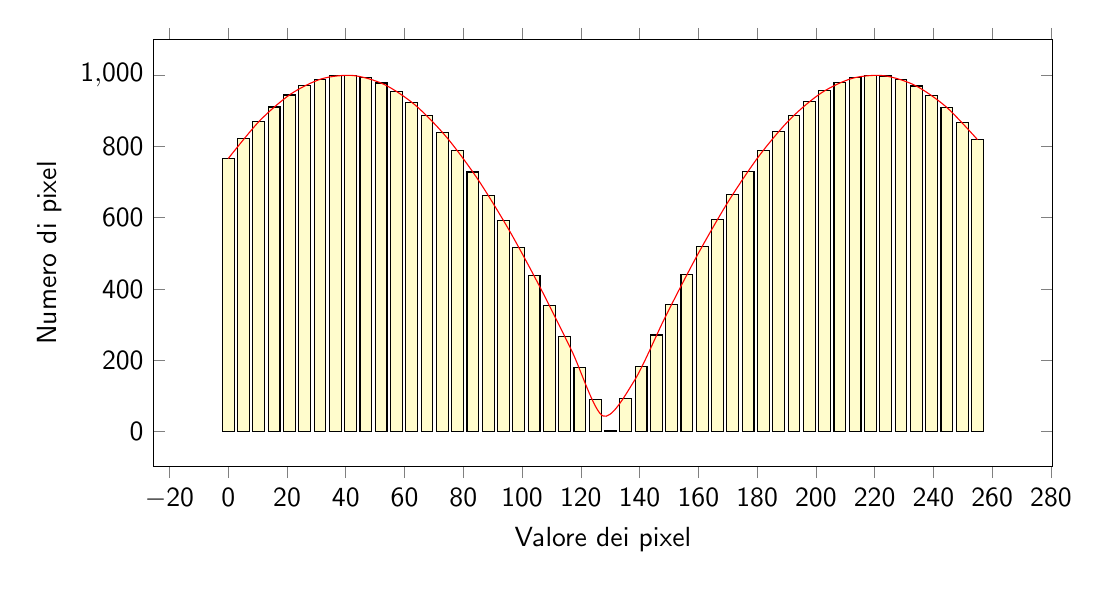
\begin{tikzpicture}[font=\sffamily]
			\begin{axis}[ybar,bar width=1.5mm,ylabel={Numero di pixel},yticklabel=$\mathsf{\pgfmathprintnumber{\tick}}$,xticklabel=$\mathsf{\pgfmathprintnumber{\tick}}$,xlabel={Valore dei pixel}]
				\addplot[samples=50,domain=0:255,fill=yellow!20] {abs(sin(x + 50)) * 1000};
				\addplot [smooth, domain=0:255, red] {abs(sin(x + 50)) * 1000};
			\end{axis}
		\end{tikzpicture}
	}
	\caption{Esempio di istogramma bimodale} \label{fig:bimodal-hist}
\end{figure}
Nel caso in cui l'immagine in analisi non presenti esattamente due massimi locali nella funzione istogramma, il procedimento di Otsu potrebbe per\`o portare a risultati indesiderati.

\section{Algoritmo di sogliatura proposto}
\label{sec:image-bin-proposed-approach}
